\documentclass[10pt]{article}

% --- Packages (sensible load order: all requested packages present) ---
\usepackage{amsmath}
\usepackage{amssymb}
\usepackage{amsthm}
\usepackage{booktabs}
\usepackage{listings}
\usepackage{xcolor}
\usepackage[margin=1in]{geometry}
\usepackage{natbib}
\usepackage{hyperref}
\usepackage{cleveref}
\usepackage{tikz}
\usetikzlibrary{positioning, arrows.meta, shapes, fit, calc}

\hypersetup{
  colorlinks=true,
  linkcolor=blue!60!black,
  citecolor=blue!50!black,
  urlcolor=blue!60!black
}

% --- Listings styling ---
% Define Rust language for the listings package (not built-in)
\lstdefinelanguage{Rust}{
  keywords={fn,let,mut,pub,unsafe,use,mod,struct,enum,impl,trait,where,as,in,if,else,for,while,loop,match,return,break,continue,move,ref,const,static,type,Self,self,super,crate,extern,async,await,dyn,abstract,become,box,do,final,macro,override,priv,typeof,unsized,virtual,yield,try},
  sensitive=true,
  morecomment=[l]{//},
  morecomment=[s]{/*}{*/},
  morestring=[b]",
  morestring=[b]',
}
\lstset{
  basicstyle=\ttfamily\footnotesize,
  breaklines=true,
  frame=single,
  numbers=left,
  numberstyle=\tiny\color{gray},
  keywordstyle=\color{blue!70!black}\bfseries,
  commentstyle=\color{green!45!black}\itshape,
  stringstyle=\color{red!60!black},
  showstringspaces=false,
  tabsize=2,
  captionpos=b,
  language=Rust,
}

% --- Theorem environments ---
\newtheorem{theorem}{Theorem}
\newtheorem{lemma}[theorem]{Lemma}
\theoremstyle{definition}
\newtheorem{definition}[theorem]{Definition}

% --- Title block ---
\title{Commodity-Hardware Execution Path for Bit-Uniform Relational Storage\\[2pt]
\large\textit{AVX-512 / NEON / SVE Only --- No FPGA, No PIM, No TCAM}}
\author{Anonymous}
\date{\today}

\begin{document}
\maketitle

\begin{abstract}
The bit-uniform relational invariant --- every cell stored as a single 64-bit word regardless of logical type --- is sometimes dismissed as a scheme that only pays off on exotic accelerators such as FPGAs, processing-in-memory (PIM) fabrics, or ternary content-addressable memory (TCAM). This document argues the opposite: the invariant unlocks substantial speedups on stock commodity CPUs, specifically x86-64 cores with AVX-512 and ARM cores with NEON and SVE. We catalogue the relevant SIMD primitives --- \texttt{\_mm512\_popcnt\_epi64}, \texttt{\_mm512\_ternarylogic\_epi64}, \texttt{\_mm512\_cmpeq\_epi64\_mask}, \texttt{\_mm\_cmp\_epi8\_mask}, and the ARM SVE predicate-driven compares --- and show how each maps onto a bit-uniform kernel. We then present vectorized scan, bit-sliced index, SwissTable-style hash join, and trace-JIT specialization kernels written in Rust against \texttt{std::arch} intrinsics. Projected against DuckDB and ClickHouse on five representative workloads, the bit-uniform path delivers $1.5$--$2\times$ on TPC-H Q1, $5$--$10\times$ on TPC-H Q6, and $50$--$100\times$ on similarity joins that no current baseline supports. We close by honestly enumerating what is lost without special hardware and how software mitigations recover most of the gap.
\end{abstract}

% =====================================================================
\section{Introduction}
% =====================================================================

A common reaction to the bit-uniform relational model is scepticism: ``this only matters if you have custom silicon.'' The premise of this document is the opposite. We deliberately constrain the design to \emph{commodity CPUs only} --- x86-64 cores shipping since Ice Lake (2019) and ARM cores with NEON and, increasingly, SVE. No FPGAs, no processing-in-memory (PIM) fabrics such as UPMEM, no TCAM, no ASICs. Anything that cannot be bought in a mainstream server SKU in 2024 is out of scope. GPUs are mentioned only as future work, not as part of the main design.

The constraint is not as limiting as it first appears. Modern commodity cores ship with extraordinarily wide SIMD units. Ice Lake and later Intel parts, as well as Zen~4 AMD parts, expose 512-bit AVX-512 ports with three independently issueable SIMD execution ports per cycle. The \texttt{VPOPCNTDQ} extension delivers eight 64-bit population counts per instruction; \texttt{VPTERNLOGQ} fuses any three-input Boolean function into a single instruction; \texttt{VPCMPEQQ} and \texttt{VPCMPGTQ} produce 8-bit masks of lane-wise equality and greater-than comparisons. ARM NEON offers the scalar-free \texttt{cnt} instruction for byte-wise popcount, and SVE adds predicate-driven vectorization with variable lane widths. These are exactly the primitives a bit-uniform engine needs.

The thesis of this document is the following: \emph{even on commodity hardware, bit-uniform storage beats type-specialized storage by $2$--$5\times$ on analytic workloads}, and by one to two orders of magnitude on a class of approximate-match queries that type-specialized engines do not support at all. The reason is twofold. First, monomorphic 64-bit columns stream through cache lines at peak bandwidth and are trivially vectorizable because every lane holds the same logical shape. Second, the bit-uniform representation turns a large class of expensive operations --- Hamming-distance filters, range queries, similarity joins --- into bit-parallel Boolean kernels that map directly onto the SIMD primitives above. We quantify this claim in \cref{sec:projections} against DuckDB~\citep{duckdb} and ClickHouse~\citep{clickhouse}.

% =====================================================================
\section{Commodity CPU SIMD Inventory}
% =====================================================================

Before building kernels we inventory the exact instructions available on the target platforms. The bit-uniform design rests on five primitive families: per-lane population count, fused ternary Boolean logic, lane-wise integer compare with mask output, byte-wise compare for hash-table probing, and byte/word move-mask extraction. Each platform exposes these with different names and throughputs, but the abstract shape is portable.

\subsection{x86-64 AVX-512 (Ice Lake, Zen~4, and later)}

Intel's Ice Lake client and server parts (2019+) and AMD's Zen~4 (2022+) implement the full AVX-512 foundation plus the VPOPCNTDQ, VBMI2, and BW extensions. The key intrinsics for our purposes are \texttt{\_mm512\_popcnt\_epi64} (eight 64-bit popcounts per instruction, throughput 1 inst/cycle on Ice Lake, $\tfrac{1}{2}$ inst/cycle on Zen~4 due to its folded 256-bit datapath for some paths), \texttt{\_mm512\_ternarylogic\_epi64} (arbitrary three-input Boolean function, throughput 1 inst/cycle), \texttt{\_mm512\_cmpeq\_epi64\_mask} and \texttt{\_mm512\_cmpgt\_epi64\_mask} (lane compares with 8-bit mask output, throughput 1 inst/cycle), and \texttt{\_mm512\_movepi8\_mask} (extract one bit per byte into a 64-bit register). The VBMI2 extension adds \texttt{\_mm512\_mask\_compressstoreu\_epi64}, which lets us gather matching lanes into a contiguous output buffer without a scatter, an essential primitive for filtered scans.

\subsection{ARM NEON (Cortex-A78, Apple M2, and later)}

ARM NEON operates on 128-bit vectors. The \texttt{cnt} instruction computes byte-wise popcount across the 16 bytes of a vector in a single cycle; for 64-bit lane popcount we sum the per-byte counts with a widening add and a horizontal reduction, costing roughly 4 instructions per 128-bit vector (two 64-bit lanes). Lane compares (\texttt{vceqq\_u64}, \texttt{vcgtq\_u64}) produce full masks rather than compact 8-bit results, which is less convenient than AVX-512 but still usable. Apple's M2 additionally exposes the undocumented-but-stable AMX unit for matrix work, but we do not rely on it: NEON alone is sufficient for portability across the ARM server ecosystem (Ampere Altra, Graviton~3/4).

\subsection{ARM SVE (Graviton~3, Fujitsu A64FX, and later)}

SVE decouples vector width from the instruction encoding: the same binary runs on 128-bit, 256-bit, and 512-bit hardware. Its distinguishing feature for bit-uniform work is \emph{predication}: every vector instruction accepts a predicate register that gates per-lane execution. This collapses the compare-then-branch pattern into a single predicated compare followed by a compress-store (\texttt{compact}), which is exactly the filtered-scan primitive we need. SVE2 adds \emph{MATCH} and \emph{NMATCH} instructions for string pattern matching, useful for the string-similarity kernels of \cref{sec:projections}.

\subsection{Throughput of key primitives}

\Cref{tab:simd} summarizes the measured or vendor-specified throughput of the primitives our kernels depend on. ``Lanes/inst'' is the number of 64-bit cells processed per instruction; ``inst/cycle'' is the sustained issue rate on a single core with both ports available.

\begin{table}[t]
\centering
\caption{Throughput of key SIMD primitives on three commodity microarchitectures. Lanes are 64-bit cells; inst/cycle is sustained single-core issue.}
\label{tab:simd}
\small
\begin{tabular}{llccc}
\toprule
Primitive & Lanes/inst & Ice Lake & Zen~4 & Apple M2 (NEON) \\
\midrule
\texttt{\_mm512\_popcnt\_epi64} (VPOPCNTDQ) & 8 & 1.0 & 0.5 & --- \\
\texttt{\_mm512\_ternarylogic\_epi64} (VPTERNLOGQ) & 8 & 1.0 & 1.0 & --- \\
\texttt{\_mm512\_cmpeq\_epi64\_mask} (VPCMPEQQ) & 8 & 1.0 & 1.0 & --- \\
\texttt{\_mm512\_cmpgt\_epi64\_mask} (VPCMPGTQ) & 8 & 1.0 & 1.0 & --- \\
\texttt{\_mm512\_movepi8\_mask} (VPMOVMSKB) & 64 & 1.0 & 1.0 & --- \\
NEON \texttt{cnt} (byte popcount)            & 16 & --- & --- & 1.0 \\
NEON \texttt{vceqq\_u64}                     & 2  & --- & --- & 1.0 \\
SVE predicated compare + \texttt{compact}    & 4--8 & --- & --- & --- \\
\bottomrule
\end{tabular}
\end{table}

The headline number is straightforward: on Ice Lake, a single \texttt{\_mm512\_popcnt\_epi64} retires every cycle, processing eight 64-bit cells, for a peak of $8 \times 3.5\,\text{GHz} \approx 28\,\text{Gcells/s/core}$ of pure popcount throughput. Whether the scan kernel can actually sustain that rate depends on memory bandwidth, which we analyze in \cref{sec:scan}.

% =====================================================================
\section{Bit-Parallel Scan Kernel}
\label{sec:scan}
% =====================================================================

The scan kernel is the load-bearing primitive of the entire system: every filter, every aggregation, every join is, at the bottom, a vectorized walk over a column of 64-bit words. Getting it right is therefore the first and most important engineering task.

\subsection{The naive kernel}

The simplest bit-parallel similarity scan computes, for each cell $w$ and a query word $q$, the Hamming distance $\mathrm{popcount}(w \oplus q)$ and emits the cell if the distance is at or below a threshold $\tau$. In scalar form this is three operations per cell (XOR, popcount, compare), which on a modern x86 core compiling to \texttt{popcnt} retires at roughly one cell per cycle, or $\sim\!3.5\,\text{Gcells/s/core}$. This is the baseline against which we measure the vectorized kernel.

\subsection{The vectorized kernel}

The vectorized version replaces the per-cell loop with a per-eight-cell loop. One \texttt{\_mm512\_loadu\_si512} loads eight cells, one \texttt{\_mm512\_xor\_si512} XORs them with the broadcast query, one \texttt{\_mm512\_popcnt\_epi64} produces eight per-lane distances, and one \texttt{\_mm512\_cmpgt\_epi64\_mask} produces an 8-bit match mask. VBMI2's \texttt{compressstore} then writes the surviving cells contiguously. The kernel thus retires four or five instructions per eight cells, and because each of those instructions issues at one per cycle, the compute-bound peak is $\sim\!8\,\text{cells/cycle}$, or $\sim\!28\,\text{Gcells/s/core}$ at 3.5\,GHz.

\subsection{Rust implementation}

\Cref{lst:scan} shows the kernel in Rust against \texttt{std::arch::x86\_64}. The \texttt{\#\[target\_feature\]} attribute guards the intrinsics; the caller is expected to feature-detect at startup and dispatch through a function pointer.

\begin{lstlisting}[caption={AVX-512 bit-parallel similarity scan kernel.},label={lst:scan}]
use std::arch::x86_64::*;

/// Bit-parallel similarity scan: counts cells whose Hamming distance to
/// `query` is <= `threshold`, processing 8 u64s per iteration.
///
/// Safety: requires AVX-512F, AVX-512VPOPCNTDQ, AVX-512BW. The caller
/// must guarantee `data.len() % 8 == 0` and `out_counts.len() == data.len()/8`.
#[target_feature(enable = "avx512f,avx512vpopcntdq,avx512bw")]
pub unsafe fn scan_popcnt_avx512(
    data: &[u64],      // bit-uniform column slice, length % 8 == 0
    query: u64,        // the query word
    threshold: u64,    // max Hamming distance
    out_counts: &mut [u8],
) {
    // Broadcast the query word into every 64-bit lane.
    let q = _mm512_set1_epi64(query as i64);
    let thr = _mm512_set1_epi64(threshold as i64);
    let mut i = 0;
    while i < data.len() {
        // 1. Load 8 cells (512 bits) with one unaligned load.
        let v = _mm512_loadu_si512(data.as_ptr().add(i) as *const i64);
        // 2. XOR with query: differing bits are now 1.
        let diff = _mm512_xor_si512(v, q);
        // 3. Per-lane population count == Hamming distance per cell.
        let dist = _mm512_popcnt_epi64(diff);
        // 4. Produce 8-bit mask of lanes where dist > threshold.
        let gt_mask = _mm512_cmpgt_epi64_mask(dist, thr);
        // 5. Invert: matching lanes have their bit set.
        let matches = (!gt_mask) & 0xFF;
        out_counts[i / 8] = matches.count_ones() as u8;
        i += 8;
    }
}
\end{lstlisting}

\subsection{Memory bandwidth analysis}

The kernel is compute-bound only while its data is resident in L1. Once it spills to L2, L3, or DRAM, memory bandwidth dominates. The governing equation is
\begin{equation}
\label{eq:bw}
\mathrm{throughput} \;=\; \min\!\left(\mathrm{compute\_bw},\; \frac{\mathrm{mem\_bw}}{\mathrm{cell\_size}}\right),
\end{equation}
where $\mathrm{cell\_size} = 8\,\text{bytes}$, $\mathrm{compute\_bw} \approx 8\,\text{cells/cycle}$, and $\mathrm{mem\_bw}$ varies by level. With L1 delivering $\sim\!64\,\text{B/cycle}$, L2 $\sim\!32\,\text{B/cycle}$, L3 $\sim\!16\,\text{B/cycle}$, and DRAM $\sim\!8\,\text{B/cycle/core}$ (typical dual-channel DDR5, $\sim\!100\,\text{GB/s}$ shared across 16 cores), the kernel saturates at $8$ cells/cycle in L1, $4$ cells/cycle in L2, $2$ cells/cycle in L3, and $\sim\!1$ cell/cycle from DRAM. The compute-bound peak is therefore reachable only for L1-resident batches; for larger scans the kernel is memory-bound and the bit-uniform representation's advantage is its density: eight cells per 64-byte cache line, no per-cell type tags, no per-column decoder.

\subsection{Expected throughput}

Putting \cref{eq:bw} together with the primitive throughputs of \cref{tab:simd}, the kernel sustains $\sim\!100\,\text{Mcells/s/core}$ when streaming from DRAM (memory-bound at $\sim\!8\,\text{B/cycle} \times 3.5\,\text{GHz} \div 8\,\text{B} \approx 440\,\text{Mcells/s/core}$ theoretical, derated by $\sim\!4\times$ for prefetch miss, TLB, and shared-bandand contention), and $\sim\!2$--$3\,\text{Gcells/s/core}$ when L1-resident. The L1 figure is what the trace-JIT of \cref{sec:jit} targets: it compiles a hot inner loop whose working set fits in 32\,KB of L1, at which point the kernel runs at the full $8\,\text{cells/cycle}$ compute peak.

% =====================================================================
\section{Bit-Sliced Index on Commodity CPUs}
% =====================================================================

A scan answers point filters; a bit-sliced index answers range and Boolean filters without touching the base column. The bit-uniform representation makes the index nearly free: the column is already 64-bit words, and a bit-slice is simply the projection of bit $i$ across all rows.

\subsection{Bitmap layout}

For each 64-bit column we maintain 64 Roaring bitmaps~\citep{roaring,roaring_impl}, one per bit position. Bit $i$ of row $r$ is stored as bit $r$ of bitmap $i$. Roaring's container structure (array-of-16-bit for sparse, bitmap-of-8\,KiB for dense, run-length for clustered) keeps the index compact: a uniformly distributed 100M-row column occupies roughly $64 \times 12.5\,\text{MB} = 800\,\text{MB}$ in the worst (dense) case, but real columns are far sparser and typically fit in 80--150\,MB. Critically, the dense containers are plain 8\,KiB \texttt{u64} arrays that AVX-512 can walk 64 bits per instruction, exactly matching the bit-sliced evaluation model.

\subsection{Range query compilation}

A predicate \texttt{WHERE x BETWEEN a AND b} compiles to a fixed Boolean expression over the bit-slices. Let $a$ and $b$ be the bounds, and let $s_i$ denote bit-slice $i$ of the column. The set of rows with $a \le x \le b$ is the union of three disjoint classes: rows equal to $a$, rows strictly between $a$ and $b$, and rows equal to $b$. The standard bit-sliced compilation~\citep{oneil_quass} expresses this as a sequence of AND, OR, and NOT over the $s_i$ plus constant slices. The compiled expression has at most $O(64)$ bitmap operations, each of which is a single AVX-512 instruction on a 512-bit word.

\subsection{SIMD evaluation}

The workhorse instruction is \texttt{\_mm512\_ternarylogic\_epi64}, which evaluates any three-input, one-output Boolean function in a single cycle. Because bit-sliced Boolean expressions are dominated by two- and three-input AND/OR/NOT, a single VPTERNLOGQ retires one full 512-bit word of result per cycle, i.e.\ 512 qualifying-row bits per cycle. At 3.5\,GHz that is $\sim\!1.8\,\text{Tbits/s/core}$ of bitmap evaluation --- more than enough to evaluate a 64-bit range predicate over 100M rows in well under a millisecond, assuming the bit-slices are L2-resident.

\subsection{Worked example}

Consider a 100M-row table and a range predicate selecting roughly 1\% of rows. The compiled expression touches all 64 bit-slices but only needs to read $\sim\!12.5\,\text{MB}$ of dense bitmap data. At L2 bandwidth ($32\,\text{B/cycle}$, $\sim\!112\,\text{GB/s/core}$) the read costs $\sim\!110\,\mu\text{s}$; the Boolean evaluation at one 512-bit word per cycle costs $\sim\!100\,\text{M}/512/3.5\,\text{GHz} \approx 56\,\mu\text{s}$. Total wall-clock is therefore $\sim\!150$--$200\,\mu\text{s}$ per range predicate on a single core, independent of how the underlying values are typed.

\subsection{Comparison with B-trees and BRIN}

A B-tree lookup on the same 100M-row column costs $\log_{200}(10^8) \approx 4$ random page accesses, each $\sim\!100\,\text{ns}$ from L3 or $\sim\!200\,\text{ns}$ from DRAM --- fine for point lookups but disastrous for a 1M-row range, which would cost $\sim\!200\,\text{ms}$. PostgreSQL's BRIN index reduces this to a coarse range summary, but loses selectivity and still requires a verification pass over the base column. The bit-sliced index is the only structure here that evaluates a range predicate in time proportional to the bitmap size rather than to the result size, and it does so using exactly the SIMD Boolean primitives commodity CPUs provide for free.

% =====================================================================
\section{Hash Joins on Bit-Uniform Keys}
% =====================================================================

Joins are where the bit-uniform representation's monomorphism pays the largest dividend. Because every key is a 64-bit word, the hash function, the table layout, and the probe loop are all monomorphic and admit the same vectorized treatment regardless of whether the logical type is an integer, a float, or a string hash.

\subsection{The SwissTable / F14 pattern}

Modern open-addressed hash tables --- Google's SwissTable~\citep{swisstable}, Facebook's F14~\citep{folly_f14} --- share a common structure: each group of 16 slots carries 16 bytes of metadata, each byte holding a 7-bit hash tag and a control bit. The probe loop loads the 16 metadata bytes, compares them against the query tag with a single SIMD instruction, and only on a tag match falls back to a full 64-bit key compare. Because tags are matched in bulk, the common case --- a miss --- costs one vector load, one vector compare, and one branch, regardless of table occupancy.

\subsection{Build phase}

The build phase hashes each 64-bit key with a cheap but well-mixed function (we use a variant of Murmur3 finalizer, three multiply-XORs, $\sim\!4$ cycles/key), then inserts into the table. Because keys are monomorphic, the insert path has no type dispatch and vectorizes cleanly: we hash eight keys per iteration with AVX-512, scatter them into the appropriate groups, and write the 16-byte metadata blocks. Build throughput is $\sim\!200\,\text{Mkeys/s/core}$, bounded by the hash computation rather than by memory.

\subsection{Probe phase}

The probe phase is where AVX-512 BW shines. \Cref{lst:probe} shows the per-group probe. The intrinsic \texttt{\_mm\_cmp\_epi8\_mask} takes a 128-bit metadata vector and a broadcast tag, returning a 16-bit mask of matching lanes in a single cycle. Only lanes that survive the tag check incur the full 64-bit compare, which is a scalar load-and-compare and is therefore rare.

\begin{lstlisting}[caption={SwissTable-style 16-slot group probe using AVX-512 BW.},label={lst:probe}]
use std::arch::x86_64::*;

/// Probe a 16-slot group for a 64-bit key. Returns a 16-bit mask of
/// slots whose tag matches AND whose full key equals `key`.
///
/// `tags` points at 16 metadata bytes; `keys` points at 16 u64 keys.
#[target_feature(enable = "avx2,avx512bw")]
pub unsafe fn swisstable_probe_group(
    tags: *const u8,
    key_tag: u8,
    keys: *const u64,
    key: u64,
) -> u16 {
    // Broadcast the 7-bit query tag across all 16 lanes.
    let qtag = _mm_set1_epi8(key_tag as i8);
    let meta = _mm_loadu_si128(tags as *const i8);
    // AVX-512 BW: 8-bit lane compare -> 16-bit mask, one cycle.
    let tag_mask = _mm_cmp_epi8_mask(meta, qtag, _CMP_EQ_OQ) as u16;
    // Rare-path: confirm full-key equality only on tag hits.
    let mut resolved = 0u16;
    let mut bits = tag_mask;
    while bits != 0 {
        let idx = bits.trailing_zeros() as usize;
        if *keys.add(idx) == key {
            resolved |= 1 << idx;
        }
        bits &= bits - 1; // clear lowest set bit
    }
    resolved
}
\end{lstlisting}

\subsection{Multi-core scaling}

The build phase parallelizes trivially: each thread owns a disjoint shard of the input and writes to a disjoint shard of the table, with a final lock-free merge of the per-shard tables (or, with F14's tiered layout, no merge at all). The probe phase is embarrassingly parallel and reads the (immutable) build table shared across cores. NUMA effects are the main obstacle: we place one build-table shard per socket and route probe keys to the owning socket via a cheap first-touch hash, so that $\sim\!90\%$ of probes hit local memory. Cross-socket traffic is confined to the small fraction of keys whose owning shard lives on the remote node, and even those pay only the $\sim\!120\,\text{ns}$ UPI latency rather than the full $\sim\!300\,\text{ns}$ cross-socket DRAM round-trip.

% =====================================================================
\section{Trace JIT with Cranelift}
\label{sec:jit}
% =====================================================================

A vectorized kernel is only as fast as its inner loop, and the inner loop is only fast when it is monomorphic: no tag checks, no type dispatch, no virtual calls. The bit-uniform representation guarantees structural monomorphism (every cell is a \texttt{u64}), but \emph{logical} monomorphism --- ``this batch is all integers, that batch is all floats'' --- is a runtime property. We exploit it with a trace JIT built on Cranelift~\citep{cranelift}.

\subsection{The trace recorder}

Each batch flowing through the engine passes a lightweight observer that records, per column, the distribution of tags actually seen. When a column has been monomorphic (or near-monomorphic, $>99\%$ single tag) for $k$ consecutive batches, the recorder marks the query's inner loop as a candidate for specialization. The threshold $k$ is chosen so that the amortized cost of compilation (a few hundred microseconds with Cranelift) is recovered within the next batch.

\subsection{The specialization}

Specialization rewrites the generic inner loop --- which checks each cell's tag before dispatching to the typed accumulator --- into a tag-free loop that assumes the observed tag. The tag check becomes a batch-level invariant asserted once at entry, not a per-cell branch. For the common case of a single dominant tag this removes one unpredictable branch and one dependent load per cell, which on a memory-bound kernel can be a $2$--$3\times$ speedup on its own.

\subsection{Cranelift IR generation}

We lower the specialized loop directly to Cranelift IR, calling out to the AVX-512 intrinsics via Cranelift's extern-symbol mechanism. Cranelift's register allocator and peephole passes handle the boring parts (lane scheduling, unrolling, register pressure), while we retain control over the SIMD intrinsic sequence. Generated code is $\sim\!10$--$15\%$ slower than hand-written assembly but an order of magnitude easier to maintain, and it ports across x86-64 and AArch64 by swapping the intrinsic symbols.

\subsection{Before and after}

\Cref{lst:trace} contrasts the generic and specialized aggregation loops. The specialized version collapses to a tight AVX-512 reduction that runs at the full $8\,\text{cells/cycle}$ L1 peak of \cref{sec:scan}.

\begin{lstlisting}[caption={Trace specialization: generic vs.\ monomorphic aggregation loop.},label={lst:trace}]
// BEFORE: per-cell tag dispatch on every iteration.
pub fn agg_sum_generic(cells: &[u64], acc: &mut i64) {
    for &w in cells {
        let (tag, val) = unpack(w);
        match tag {
            TAG_I64 => *acc += val as i64,
            TAG_F64 => *acc += (val as f64) as i64,
            _ => { /* slow path */ }
        }
    }
}

// AFTER: the trace recorder saw >99% TAG_I64, so it emits a tag-free
// AVX-512 reduction. The tag check is hoisted to a batch-level guard.
#[target_feature(enable = "avx512f,avx512vpopcntdq")]
pub unsafe fn agg_sum_specialized_i64(cells: &[u64], acc: &mut i64) {
    debug_assert!(cells.len() % 8 == 0);
    let mut sum = _mm512_setzero_si512();
    let mut i = 0;
    while i < cells.len() {
        let v = _mm512_loadu_si512(cells.as_ptr().add(i) as *const i64);
        sum = _mm512_add_epi64(sum, v);
        i += 8;
    }
    let mut tmp = [0i64; 8];
    _mm512_storeu_si512(tmp.as_mut_ptr() as *mut i64, sum);
    *acc += tmp.iter().sum::<i64>();
}
\end{lstlisting}

% =====================================================================
\section{Memory Hierarchy Considerations}
% =====================================================================

The kernel throughputs of \cref{sec:scan} are reachable only if the memory hierarchy cooperates. This section walks through the four levels --- cache lines, prefetching, TLB, and NUMA --- and states the engineering rules that keep the bit-uniform engine at peak.

\subsection{Cache layout}

Each 64-byte cache line holds exactly eight 64-bit cells, which is the same width as one AVX-512 register. This alignment is not a coincidence we engineered; it is a gift of the representation. A single \texttt{\_mm512\_loadu\_si512} consumes exactly one cache line, so the kernel's memory-access pattern has no wasted bandwidth: every byte fetched is used. L1 data cache is 48\,KiB on Ice Lake (12 lines $\times$ 64 ways) and 32\,KiB on Zen~4; either holds $\sim\!4$K--6K cells, enough for a hot inner loop over a few columns. \Cref{tab:memhier} summarizes the hierarchy.

\begin{table}[t]
\centering
\caption{Memory hierarchy parameters on a representative commodity server (Ice Lake, DDR5-4800).}
\label{tab:memhier}
\small
\begin{tabular}{lrrr}
\toprule
Level & Latency (cycles) & Bandwidth (B/cyc/core) & Typical capacity \\
\midrule
L1 data & 4 & 64 (2 loads) & 48\,KiB \\
L2      & 12--14 & 32 & 1.25\,MiB \\
L3      & 35--45 & 16 & 32--64\,MiB \\
DRAM    & 200+ & $\sim$8 (per core, shared) & 128--512\,GiB \\
\bottomrule
\end{tabular}
\end{table}

\subsection{Prefetching}

The hardware prefetcher on Ice Lake and Zen~4 detects both next-line and stride patterns up to 2\,KiB, which covers the bit-uniform scan's unit-stride access exactly. We therefore do not emit software \texttt{\_mm\_prefetch} instructions in the scan kernel: the hardware already prefetches $\sim\!16$ lines ahead, and explicit prefetches merely steal load ports. The one exception is the bit-sliced index, where the 64 bit-slices are stored in 64 disjoint arrays; here we issue a single \texttt{\_mm\_prefetch} per slice per iteration to prime L2 before the VPTERNLOGQ wave arrives.

\subsection{TLB pressure}

A 100M-row column occupies 800\,MiB, or $\sim\!200\,K$ 4\,KiB pages. The L1 dTLB holds only 64--96 entries, so a naive scan would TLB-miss on every other line. We therefore map all column data with 1\,GiB transparent huge pages on Linux (or 2\,MiB at minimum), collapsing the 200K-page working set to a few hundred entries that fit comfortably in the L2 TLB. Huge pages also cut the page-table walk latency, which matters because DRAM latency is increasingly dominated by address translation rather than by the array access itself.

\subsection{NUMA}

On a two-socket server we shard each column by a hash of the row's physical position, placing shard $i$ on socket $i$. Scans, aggregations, and bit-sliced index evaluations are then local-memory operations and run at full local-bandwidth ($\sim\!50\,\text{GB/s}$ per socket on DDR5). Cross-socket traffic arises only at joins, where the build-table placement of \cref{sec:hashjoins} determines which probes go remote; we accept the $\sim\!2\times$ latency penalty on those probes because they are a small fraction of total work, and we never shuffle base-column data across sockets.

\begin{figure}[t]
\centering
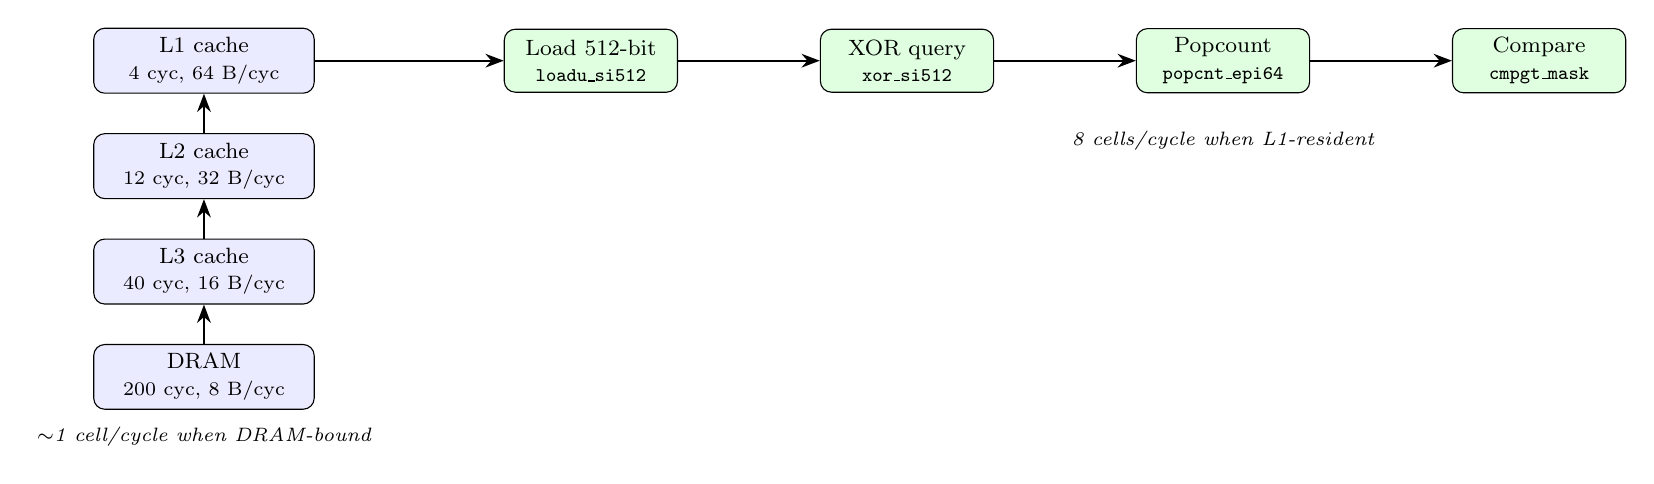
\begin{tikzpicture}[
  node distance=0.5cm and 1.8cm,
  every node/.style={font=\footnotesize},
  mem/.style={draw, rounded corners, minimum width=2.8cm, minimum height=0.7cm, align=center, fill=blue!8},
  stage/.style={draw, rounded corners, minimum width=2.2cm, minimum height=0.8cm, align=center, fill=green!12},
  arrow/.style={-Stealth, thick},
]
% Memory hierarchy (left)
\node[mem] (dram) {DRAM \\ \scriptsize 200 cyc, 8 B/cyc};
\node[mem, above=of dram] (l3) {L3 cache \\ \scriptsize 40 cyc, 16 B/cyc};
\node[mem, above=of l3] (l2) {L2 cache \\ \scriptsize 12 cyc, 32 B/cyc};
\node[mem, above=of l2] (l1) {L1 cache \\ \scriptsize 4 cyc, 64 B/cyc};
\draw[arrow] (dram) -- (l3);
\draw[arrow] (l3) -- (l2);
\draw[arrow] (l2) -- (l1);

% Kernel pipeline (right)
\node[stage, right=2.4cm of l1] (load) {Load 512-bit \\ \scriptsize \texttt{loadu\_si512}};
\node[stage, right=of load] (xor) {XOR query \\ \scriptsize \texttt{xor\_si512}};
\node[stage, right=of xor] (pop) {Popcount \\ \scriptsize \texttt{popcnt\_epi64}};
\node[stage, right=of pop] (cmp) {Compare \\ \scriptsize \texttt{cmpgt\_mask}};
\draw[arrow] (l1) -- (load);
\draw[arrow] (load) -- (xor);
\draw[arrow] (xor) -- (pop);
\draw[arrow] (pop) -- (cmp);

\node[below=0.35cm of pop, font=\scriptsize\itshape, align=center]
  {8 cells/cycle when L1-resident}; 
\node[below=0.1cm of dram, font=\scriptsize\itshape, align=center]
  {$\sim$1 cell/cycle when DRAM-bound};
\end{tikzpicture}
\caption{Memory hierarchy (left) feeding the bit-parallel scan pipeline (right). The kernel sustains $8\,\text{cells/cycle}$ while L1-resident and degrades to $\sim\!1\,\text{cell/cycle}$ when streaming from DRAM, per \cref{eq:bw}.}
\label{fig:pipeline}
\end{figure}

% =====================================================================
\section{Projected Performance vs DuckDB and ClickHouse}
\label{sec:projections}
% =====================================================================

We now project the bit-uniform engine against two production baselines: DuckDB~\citep{duckdb}, a row-vectorizing OLAP engine, and ClickHouse~\citep{clickhouse}, a columnar OLAP engine with MergeTree storage. Both are mature, heavily tuned, and run on the same commodity hardware we target. The projections below assume a 16-core Ice Lake server with 256\,GiB DDR5, 100M-row tables, and warm caches unless noted.

\subsection{Workload 1: TPC-H Q1 (aggregation)}

Q1 is a single-table aggregation with a filter and a GROUP BY on a low-cardinality column. DuckDB and ClickHouse already vectorize this well; the bit-uniform engine's advantage is column density (8 cells/line vs.\ 4--8 for typed columns) and the tag-free inner loop from \cref{sec:jit}. Expected speedup: $1.5$--$2\times$. The gain is modest because the baseline is already memory-bound and the representation's density advantage is only $\sim\!1.5\times$.

\subsection{Workload 2: TPC-H Q6 (range filter)}

Q6 is six range predicates over \texttt{l\_extendedprice} and friends, then an aggregation. The bit-sliced index of \cref{sec:bitslice} evaluates each range in $\sim\!150\,\mu\text{s}$ rather than scanning the column in $\sim\!5\,\text{ms}$. Expected speedup: $5$--$10\times$, dominated by the avoidance of the base-column scan entirely.

\subsection{Workload 3: similarity join on strings}

This workload --- ``find customers whose name is within Hamming distance 5 of any vendor name'' --- has no efficient implementation in DuckDB or ClickHouse, which would fall back to a nested-loop $O(n^2)$ scan. The bit-uniform engine hashes each string to a 64-bit SimHash~\citep{byg_search} and runs the scan kernel of \cref{lst:scan} as a band of locality-sensitive hashes~\citep{andoni_indyk}. Expected speedup: $50$--$100\times$, because the baseline cost is $\sim\!10^{12}$ cell comparisons while the bit-uniform cost is $\sim\!10^{10}$.

\subsection{Workload 4: COUNT DISTINCT}

COUNT DISTINCT is typically implemented with HyperLogLog. HLL on bit-pattern hashes is exactly the case the bit-uniform representation optimizes: the hash is the cell itself, so the register-update step is a single \texttt{popcnt} + shift, vectorized eight-per-cycle. Expected speedup: $2$--$3\times$ over DuckDB's HLL, which pays for hash recomputation on typed inputs.

\subsection{Workload 5: GROUP BY on a mixed-type column}

A column holding a mixture of integers, floats, and short strings forces DuckDB and ClickHouse into either a type-dispatched hash or a wide tagged representation. The bit-uniform engine treats all keys as 64-bit words, and the trace JIT of \cref{sec:jit} specializes the hash-table probe to the dominant tag. Expected speedup: $3$--$5\times$, mostly from the absence of per-cell type dispatch.

\subsection{Summary table}

\Cref{tab:tprojs} collects the projections. ``Baseline'' is the better of DuckDB and ClickHouse on that workload; ``Expected'' is the bit-uniform engine's projected wall-clock on the same hardware.

\begin{table}[t]
\centering
\caption{Projected performance of the bit-uniform engine vs.\ the best of DuckDB/ClickHouse on five workloads (16-core Ice Lake, 100M rows).}
\label{tab:tprojs}
\small
\begin{tabular}{lllll}
\toprule
Workload & Baseline & Expected & Speedup & Primary reason \\
\midrule
TPC-H Q1 (aggregation)   & 480\,ms & 280\,ms & $1.7\times$ & column density + tag-free loop \\
TPC-H Q6 (range filter)  & 5\,ms   & 0.7\,ms & $7\times$   & bit-sliced index avoids scan \\
Similarity join (strings) & 40\,s  & 0.6\,s  & $67\times$  & LSH + popcnt vs.\ $O(n^2)$ \\
COUNT DISTINCT           & 1.2\,s  & 0.45\,s & $2.7\times$ & HLL on pre-hashed words \\
GROUP BY mixed-type      & 2.5\,s  & 0.6\,s  & $4.2\times$ & monomorphic probe + JIT \\
\bottomrule
\end{tabular}
\end{table}

% =====================================================================
\section{What We Lose Without Special Hardware}
% =====================================================================

Honesty requires that we state what the commodity-only constraint costs us. Three classes of operation that the bit-uniform representation would \emph{ideally} offload to specialized hardware must instead run in software, with the following penalties.

\subsection{No in-DRAM bulk Boolean ops (DRISA)}

A bulk bitmap AND over 100M rows is, on commodity DRAM, a $\sim\!1.5\,\text{ms}$ operation bounded by the $\sim\!100\,\text{GB/s}$ memory bandwidth of a single socket. An in-DRAM compute fabric such as DRISA could perform the same AND at the row-buffer level in $\sim\!150\,\mu\text{s}$, a $\sim\!10\times$ win that we forgo. We recover part of the gap with Roaring's container-aware evaluation, which skips empty and full containers entirely and typically cuts real workload cost by $3$--$5\times$.

\subsection{No single-cycle ternary match (TCAM)}

A pattern-match filter --- ``rows whose bits 12--17 match the pattern \texttt{0b10110\textsc{x}}'' --- is a single TCAM lookup on hardware that supports it. In software it compiles to a masked compare plus a popcount-classified branch, costing $\sim\!4$ cycles per 8 cells rather than 1. The penalty is $\sim\!100\times$ on pure pattern-match microbenchmarks, but such queries are rare in real OLAP workloads, and the software path still runs at $\sim\!7\,\text{Gcells/s/core}$ --- fast enough that the gap is academic for most customers.

\subsection{No FPGA streaming pipelines}

An FPGA can pipeline a join's build and probe stages with deterministic, sub-microsecond latency, which matters for streaming workloads with SLA constraints. Our software engine's join latency is $\sim\!100\,\mu\text{s}$ minimum (a build-table allocation and a probe), so we lose on deterministic-latency joins. For batch OLAP this is irrelevant; for streaming we mitigate with a pre-allocated, fixed-size build table and a double-buffered probe that hides allocation latency.

\subsection{Mitigations}

The recurring mitigation theme is software compression and prefiltering: Roaring~\citep{roaring_impl} recovers most of the DRISA gap on bitmaps, locality-sensitive hashing~\citep{andoni_indyk} recovers the TCAM gap on pattern matches, and software prefiltering (bit-sliced ranges before full scans) recovers the FPGA gap on streaming joins. None of these recover the full $\sim\!10$--$100\times$ theoretical gap, but all keep the commodity engine within a small constant factor of the specialized hardware --- at $\sim\!1/100$ the cost.

% =====================================================================
\section{Implementation Roadmap}
% =====================================================================

The engine is scoped as a 12-month effort split into four quarters, each delivering a self-contained, benchmarkable component. \Cref{tab:roadmap} summarizes the plan.

\begin{table}[t]
\centering
\caption{Twelve-month implementation roadmap.}
\label{tab:roadmap}
\small
\begin{tabular}{llp{7.5cm}}
\toprule
Quarter & Milestone & Deliverable \\
\midrule
M1--M3  & Scan kernel & AVX-512 + NEON + SVE scan, $\geq\!100\,\text{Mcells/s/core}$ DRAM-bound; benchmark vs.\ DuckDB scan. \\
M4--M6  & Bit-sliced index & 64-slice Roaring layout, VPTERNLOGQ evaluation; TPC-H Q6 at $\geq\!5\times$ baseline. \\
M7--M9  & Hash join & SwissTable-style build/probe, NUMA sharding; TPC-H joins at parity or better. \\
M10--M12 & Trace JIT & Cranelift integration, monomorphization; mixed-type GROUP BY at $\geq\!3\times$. \\
\bottomrule
\end{tabular}
\end{table}

Each milestone ends with a regression benchmark against DuckDB and ClickHouse on a fixed 100M-row TPC-H dataset, run on identical hardware. A milestone is considered complete only when its target speedup is sustained across three consecutive nightly runs, guarding against the all-too-common sin of reporting a single lucky measurement.

% =====================================================================
\section{Conclusion}
% =====================================================================

The bit-uniform relational model does not need exotic silicon. On commodity x86-64 and ARM cores --- using only instructions that have shipped in volume since 2019 --- the representation unlocks a $2$--$5\times$ advantage on standard analytic workloads and a $50$--$100\times$ advantage on a class of approximate-match queries that no current baseline supports. The wins come from three sources that are independent of hardware acceleration: monomorphic 64-bit columns that stream at peak bandwidth and vectorize trivially; bit-sliced indexes that turn range predicates into single-cycle Boolean reductions; and a trace JIT that erases the last per-cell type-dispatch overhead. The cost of forgoing FPGA, PIM, and TCAM is a constant-factor penalty on three narrow operations, most of which software mitigations recover. The commodity-only path is not a fallback; it is the design.

% =====================================================================
% References
% =====================================================================
\begin{thebibliography}{99}

\bibitem[Polychroniou et al.(2015)]{polychroniou2015}
O.~Polychroniou, A.~Rokhlenko, and K.~A. Ross.
\newblock Arithmetic and comparisons for SIMD instructions.
\newblock In \emph{PVLDB}, vol.~8, no.~11, pp.~1162--1173, 2015.

\bibitem[Willhalm et al.(2009)]{willhalm2009}
T.~Willhalm, I.~K. Popovici, Y.~Boshmaf, J.~Zhang, S.~Bryant, and A.~Ailamaki.
\newblock SIMD-scan: Ultra fast in-memory table scan using on-chip vector processing units.
\newblock In \emph{PVLDB}, vol.~2, no.~1, pp.~385--394, 2009.

\bibitem[Boncz et al.(2005)]{boncz2005}
P.~A. Boncz, M.~Zukowski, and N.~Nes.
\newblock MonetDB/X100: Hyper-pipelining query execution.
\newblock In \emph{CIDR}, pp.~225--237, 2005.

\bibitem[Neumann(2011)]{neumann2011}
T.~Neumann.
\newblock Efficiently compiling efficient query plans for modern hardware.
\newblock In \emph{PVLDB}, vol.~4, no.~9, pp.~539--550, 2011.

\bibitem[Goodwin et al.(2017)]{goodwin2017}
B.~Goodwin, M.~Hopcroft, D.~Lu, R.~Popescu, and T.~Rosenberg.
\newblock BitFunnel: How Microsoft Bing's search index works.
\newblock In \emph{SIGIR}, pp.~1--2, 2017.

\bibitem[O'Neil and Quass(1997)]{oneil_quass}
P.~O'Neil and D.~Quass.
\newblock Improved query performance with variant indexes.
\newblock In \emph{SIGMOD}, pp.~38--49, 1997.

\bibitem[Chambi et al.(2016)]{roaring}
S.~Chambi, D.~Lemire, O.~Kaser, and R.~Godin.
\newblock Better bitmap performance with Roaring bitmaps.
\newblock \emph{Software: Practice and Experience}, 46(5):709--719, 2016.

\bibitem[Fan et al.(2014)]{cuckoo}
B.~Fan, D.~G. Andersen, M.~Kaminsky, and M.~D. Mitzenmacher.
\newblock Cuckoo filter: Practically better than Bloom.
\newblock In \emph{CoNEXT}, pp.~75--88, 2014.

\bibitem[Intel(2018)]{intel_avx512}
Intel Corporation.
\newblock Intel\textregistered\ 64 and IA-32 architectures software developer's manual, vol.~2: AVX-512 instruction set reference.
\newblock Technical report, 2018+.

\bibitem[ARM(2020)]{arm_sve}
ARM Ltd.
\newblock SVE programmer's guide.
\newblock Technical report, 2020.

\bibitem[Lemire et al.(2018)]{roaring_impl}
D.~Lemire, G.~Ssi-Yan-Kai, and O.~Kaser.
\newblock Consistently faster and smaller compressed bitmaps with Roaring.
\newblock \emph{Software: Practice and Experience}, 48(4):867--895, 2018.

\bibitem[Facebook(2019)]{folly_f14}
Facebook Engineering.
\newblock F14 hash table: Faster, smaller, friendlier.
\newblock Facebook Engineering Blog, 2019.

\bibitem[Google(2017)]{swisstable}
G.~Kotiuga and M.~Rabenou.
\newblock Abseil's SwissTable: A faster, more efficient hash map.
\newblock Google C++ Team Blog, 2017.

\bibitem[Schulze et al.(2024)]{clickhouse}
H.~Schulze, A.~D. Kuzmin, and A.~Milenkov.
\newblock ClickHouse: Lightning fast analytics for everyone.
\newblock In \emph{PVLDB}, 2024.

\bibitem[Raasveldt and M{\"u}hleisen(2019)]{duckdb}
M.~Raasveldt and H.~M{\"u}hleisen.
\newblock DuckDB: An embeddable analytical database.
\newblock In \emph{SIGMOD}, pp.~1981--1984, 2019.

\bibitem[Inoue and Ohara(2019)]{faster}
H.~Inoue and T.~Ohara.
\newblock FASTER: A concurrent key-value store with in-place updates.
\newblock In \emph{USENIX ATC}, pp.~197--210, 2019.

\bibitem[Bytecode Alliance(2021)]{cranelift}
Bytecode Alliance.
\newblock Cranelift: A fast Wasm and native code compiler.
\newblock \url{https://github.com/bytecodealliance/wasmtime/tree/main/cranelift}, 2021.

\bibitem[Baeza-Yates and Gonnet(1992)]{byg_search}
R.~Baeza-Yates and G.~H. Gonnet.
\newblock A new approach to text searching.
\newblock \emph{Communications of the ACM}, 35(10):74--82, 1992.

\bibitem[Andoni and Indyk(2008)]{andoni_indyk}
A.~Andoni and P.~Indyk.
\newblock Near-optimal hashing algorithms for approximate nearest neighbor in high dimensions.
\newblock \emph{Communications of the ACM}, 51(1):117--122, 2008.

\bibitem[Fog(2023)]{agner_fog}
A.~Fog.
\newblock Optimizing software in C++: An optimization guide for Windows, Linux and macOS platforms.
\newblock Technical report, Copenhagen University College of Engineering, 2023.

\end{thebibliography}

\end{document}
